\documentclass[prb,9pt,notitlepage]{revtex4-1}
%\documentclass[a4paper,twocolumn,9pt]{article}

%\usepackage{geometry}
%\geometry{a4paper,top=2.5cm,bottom=2cm,inner=1.5cm,outer=1.5cm}

\usepackage{mwe}% just for the example content
\usepackage{color}
\usepackage{latexsym,amsmath}
\usepackage{physics}
\usepackage{listings}
\usepackage[dvipsnames]{xcolor}
\usepackage{parskip}
\usepackage{hyperref}
%\usepackage{dblfloatfix}
%\usepackage{subfig}
\definecolor{linkcolor}{rgb}{0,0,0.65}%hyperlink
\definecolor{shadecolor}{rgb}{0.93, 0.93, 0.93}
%\usepackage[pdftex,colorlinks=true, pdfstartview=FitV, linkcolor= linkcolor, citecolor= linkcolor, urlcolor= linkcolor, hyperindex=true,hyperfigures=true]{hyperref} %hyperlink%
%\usepackage[backend=biber, sorting=ynt]{biblatex}
%\usepackage{ragged2e} % to justify caption
%\addbibresource{bibliography.bib}
 \usepackage{booktabs}

\usepackage[T1]{fontenc}
\usepackage{xcolor}
\usepackage{lmodern}
\usepackage{listings}
\lstset{language=[95]Fortran,
  backgroundcolor=\color{shadecolor},
  basicstyle=\ttfamily,
  keywordstyle=\color{blue},
  commentstyle=\color{gray},
  stringstyle=\color{red},
  showstringspaces=false
  %morecomment=[l]{!\ }% Comment only with space after !
}

\usepackage{tabularx}

\usepackage{fancyhdr}
\pagestyle{fancyplain}% <- use fancyplain instead fancy
\fancyhf{}
\fancyhead[R]{\today}
\fancyhead[L]{Alessandro Lambertini}
\fancyfoot[L]{Quantum information and computing}
\fancyfoot[C]{Report 2}
\fancyfoot[R]{\thepage}

\renewcommand{\headrulewidth}{0pt}

\usepackage{float}
\usepackage{siunitx}




\begin{document}
\title{Quantum information and computing: Exercises report, week 4. \\ Multi-run script \& Automated fits }

\author{Alessandro Lambertini}


\date{\today}

\begin{abstract}
Through the exercises of this week, we try to implement a program to solve the diagonalization problem for an hermitian random matrix and to study its properties. In particular, we have to compute, in different ways, the normalized spacing between neighboring eigenvalues and study these distributions. We have to do this not only for an hermitian matrix but also for a diagonal matrix with random real entries.
\end{abstract}

\maketitle

\section{Theory}
\subsection{Hermitian matrices}
An hermitian matrix is a complex square matrix that is equal to its own conjugate transpose. Some ways to caracterize these matrices are:

\begin{eqnarray}
  A \ hermitian \Longleftrightarrow \ A = \bar{A^T} \nonumber \\
  A \ hermitian \Longleftrightarrow \ a_{ij} = \bar{a_{ji}} \nonumber\\
  A \ hermitian \Longleftrightarrow \ (v,Aw) = (Av,w) \nonumber
\end{eqnarray}
\\
The eigenvalues of these matrices are, as their diagonal entries, all real. They are expecially important for their role in quantum mechanics, in the Copenhagen interpretation.
To Solve the diagonalization problem with respects to this kind of matrices in Fortran we exploit the \textit{lapack} library, which stand for \textit{linear algebra PACKage}, that is a package written in Fortran90 that provides a lot of subroutines useful for solving systems of simultaneous linear equations, least-squares solutions of linear systems of equations, eigenvalue problems, and singular value problems. In particular, we exploit the \textit{zheev()} subroutine, which coumputes all the eigenvalues and, optionally, the eigenvector of a given  complex Hermitian matrix.

\subsection{spacing}
Spacing between neighboring eigenvalues is defined by:
\begin{equation}
  s_i = \Delta \lambda / \bar{\Delta \lambda} = \frac{\lambda_{i+1}-\lambda_i}{\frac{1}{N-1}\sum_{i=1}^{N-1}(\lambda_{i+1}-\lambda_i)} \nonumber
\end{equation}
Where $N$ is the dimension of the matrix, and so the number of eigenvalues.

The distribution of the $s_i$ should follow two different approximations that came from the application, by Eugene Wigner, of random matrices to the study of the spaces between points in the spectra of nuclei of heavy atoms. These approximations, that go under the name 'Wigner surmise', are:
\begin{equation}
  P_w(s) = \frac{\pi s}{2}e^{-\pi s^2/4} \label{wigner1}
\end{equation}
which is exact for 2X2 real symmetric matrices, with elements that are i.i.d. standard gaussian random variables, and a good aproximation for matrices of any dimension. Then,
\begin{equation}
  P(s) = \frac{32s^2}{\pi^2}e^{-4s^2/\pi} \label{wigner2}
\end{equation}
which is the corresponding result for complex hermitian matrices.




\section{Code development}
In order to implement and test all the code requested in the exercises I wrote a module named \textit{ex05module} where are located all the subroutines useful to solve the different tasks. The first thing we are required to do is to initialize a random hermitian matrix and diagonalize it, storing the resulting eigenvalues and eigenvectors in a proper way. In order to do so, after having implemented the subroutine \textit{rand\_init\_hermit\_mat(mm,dim\_1,debug)} that initialize this kind of matrices, I exploit the \textit{zheev()} laPACK's subroutine to solve the diagonalization problem writing the following subroutine:
\begin{lstlisting}
subroutine diag_hermit_matrix(matrix,eigv)
  complex(kind=8), allocatable :: work(:)
  complex(kind=8), dimension(:,:) :: matrix
  integer, dimension(2) :: dimm
  integer :: msize, lwork, info
  double precision, allocatable :: rwork(:), eigv(:)

  dimm = shape(matrix)
  msize = dimm(1)

  allocate(eigv(msize))
  allocate(work(msize*msize))
  allocate(rwork(3*msize-2))
  lwork = msize*msize

  call zheev('N','L',msize,matrix,msize,eigv,work,-1,rwork,info)
  lwork = work(1)   !set the best value for lwork

  call zheev('V','L',msize,matrix,msize,eigv,work,lwork,rwork,info)

  !exploit the zheev() debug flag
  if (info.gt.0) then
    write(*,*)'The algorithm failed to compute eigenvalues.'
  end if
end subroutine diag_hermit_matrix
\end{lstlisting}
This subroutine set the parameters of \textit{zheev()} properly for what we have to do, check for the convergence of the diagonalization process and store the eigenvalues, in ascending order, in the array \textit{'eigv'}. Finally, it transform the input matrix in its diagonal form.
\\ \\
After that, we have to compute the spacing between the eigenvalues. To accomplish this result I implemented two different subroutines, the first computes the average $\bar{\Delta \lambda}$  between all the eigenvalues differences, the second one instead computes the average spacing $\bar{\Delta \lambda}$ locally, i.e., over a different number of levels around $\lambda_i$. Since the first subroutine is pretty trivial, here i report only the second one:
\begin{lstlisting}
!!!!!!!!!!!!!!!!!!!!! moving average Spacing!!!!!!!!!!!!!!!!!!!!
subroutine mov_av_norm_spacing(eigv,spacing_vec,N)
real(kind=8), allocatable :: spacing_vec(:)
real(kind=8), dimension(:) :: eigv
real(kind=8) :: av_delta
integer :: i, j, N

allocate(spacing_vec(size(eigv)-1))
av_delta = 0
!compute the eigenvalues difference
do i=1,size(spacing_vec)
  spacing_vec(i) = eigv(i+1)-eigv(i)
  if (abs(spacing_vec(i)) < 1e-15) then
    spacing_vec(i) = 0
  end if
end do
!compute the average (av_delta)
do i=1,size(spacing_vec)
  av_delta = 0
  !sufficient number of eigenvalues both right and left
  if ((i > N/2) .and. (i<size(spacing_vec)-N/2)) then
    do j=(i-N/2),(i+N/2)
      av_delta=av_delta+spacing_vec(j)
    end do

    av_delta = av_delta/N

    spacing_vec(i) = spacing_vec(i)/av_delta

  !insufficient number of eigenvalues to the left
  else if (i.le.N/2) then
    av_delta = sum(spacing_vec(1:N))/N
    spacing_vec(i) = spacing_vec(i)/av_delta

  !insufficient number of eigenvalues to the right
  else if(i.ge.size(spacing_vec)-1-N/2) then
    av_delta = sum(spacing_vec(size(spacing_vec)-N:size(spacing_vec)))/N
    spacing_vec(i) = spacing_vec(i)/av_delta
  end if
end do
end subroutine mov_av_norm_spacing
!!!!!!!!!!!!!!!!!!!!!!!!!!!!!!!!!!!!!!!!!!!!!!!!!!!!!!!!!!!
\end{lstlisting}
This subroutine takes as arguments the eivenvalues array, an array where to store the spacing values and $N$, the number of levels to use to compute the mean around $\Delta\lambda_i$. If the number of levels is sufficient both to the right and to the left of the considered eigenvalues difference, then the subroutine computes the mean centered on it. If this is not the case, the subroutine keeps the first, or the last, N $\Delta \lambda_i$ to compute the mean.

Once the array with all the spacing is obtained we can compute their distribution with the \textit{PDF\_vec} subroutine, which essentially compute the histogram (normalized or not) of a given dataset, once the number of bins is provided:
\begin{lstlisting}
!!!!!!!!! compute the distribution of the elements of a real vector !!!!!!!!
subroutine PDF_vec(spacing_vec, N_bins, bins_centers, probs, norm)
real(kind=8), dimension(:) :: spacing_vec
real(kind=8), dimension(:), allocatable :: probs, bins_centers, counts,bins_edges
integer :: N_bins, i, j
real(kind=8) :: area, ds
logical :: norm

allocate(probs(N_bins), bins_centers(N_bins), &
         counts(N_bins),bins_edges(N_bins+1))

!bins definition
ds = (maxval(spacing_vec)-minval(spacing_vec))/N_bins

do i=1,N_bins
  bins_centers(i) = minval(spacing_vec) + (i - 0.5)*ds
end do

do i=1,N_bins+1
  bins_edges(i) = minval(spacing_vec) + (i-1)*ds
end do

!counting procedure
counts = 0
do i=1,size(spacing_vec)
  do j=1,N_bins
    if ((spacing_vec(i).ge.bins_edges(j)) .and. &
    (spacing_vec(i).le.bins_edges(j+1))) then
      counts(j)=counts(j)+1
    end if
  end do
end do

if (norm .eqv. .true.) then
  area= sum(counts*ds)
  probs = counts/area
else if (norm .eqv. .false.) then
  probs = counts
end if
end subroutine PDF_vec
!!!!!!!!!!!!!!!!!!!!!!!!!!!!!!!!!!!!!!!!!!!!!!!!!!!!!!!!!!!
\end{lstlisting}
From this subroutine we obtain two arrays. The first one, \textit{bins\_centers} representing the mid point of each bin that form the histogram, will be used as the source of the x-axis values of our data. The second one, \textit{probs}, instead represents either the counts or the probabilities, depending on the value of \textit{norm}, accumulated in each bin.

Moreover, we have to fit the obtained distributions, for an hermitian matrix, and for a diagonal matrix with random real entries, with the particular model:
\begin{equation}
  P(s) = as^{\alpha}e^{-bs^{\beta}}
\end{equation}
which closely recalls the Wigner surmise (\ref{wigner1}) and (\ref{wigner2}). To do so, I exploited the gnuplot script implemented for the previous exercises and pass to it the different \textit{.csv} files obtained in the main program \textit{Ex\_05.f90}.

Finally, we have to compute the average $<r>$ of the following quantities:
\begin{equation}
  r_i = \frac{\mbox{min}(\Delta\lambda_i,\Delta\lambda_{i+1})}{\mbox{max}(\Delta\lambda_i,\Delta\lambda_{i+1})}
\end{equation}
Therefore, I implemented the following subroutine to compute it:
\begin{lstlisting}
!!!!!!!!!!!!!!!!!!!! Compute <r> !!!!!!!!!!!!!!!!!!!!
subroutine compute_r_mid(eigv,r_mid)
real(kind=8), allocatable :: spacing_vec(:), rr(:)
real(kind=8), dimension(:) :: eigv
real(kind=8) :: r_mid
integer :: i

allocate(spacing_vec(size(eigv)-1), rr(size(eigv)-2))

!compute spacing_vec without normalization
do i=1,size(spacing_vec)
  spacing_vec(i) = eigv(i+1)-eigv(i)
  if (abs(spacing_vec(i)) < 1e-15) then
    spacing_vec(i) = 0
  end if
end do

!compute r_i
do i=1,size(rr)
  rr(i) = min(spacing_vec(i),spacing_vec(i+1))/max(spacing_vec(i), &
              spacing_vec(i+1))
end do

!compute the average <r>
r_mid = sum(rr)/size(rr)
end subroutine compute_r_mid
!!!!!!!!!!!!!!!!!!!!!!!!!!!!!!!!!!!!!!!!!!!!!!!!!
\end{lstlisting}

\section{Results}
In \ref{fig:foobar} are reported some of the fits produced, with $N$, the dimension of the matrices, equal to $5000$ and the number of bins for the histograms equal to $71$. It is possible to appreciate the different distributions for hermitian and random diagonal real matrices. The effect of the moving average approach in computing $\bar{\Delta\lambda}$ is relevant in both cases with opposite effects: reducing the number of samples used to compute the average stretches the distribution in the hermitian case, while, in the diagonal case, it seems to crushes the distribution to zero.

\begin{figure}[H]
    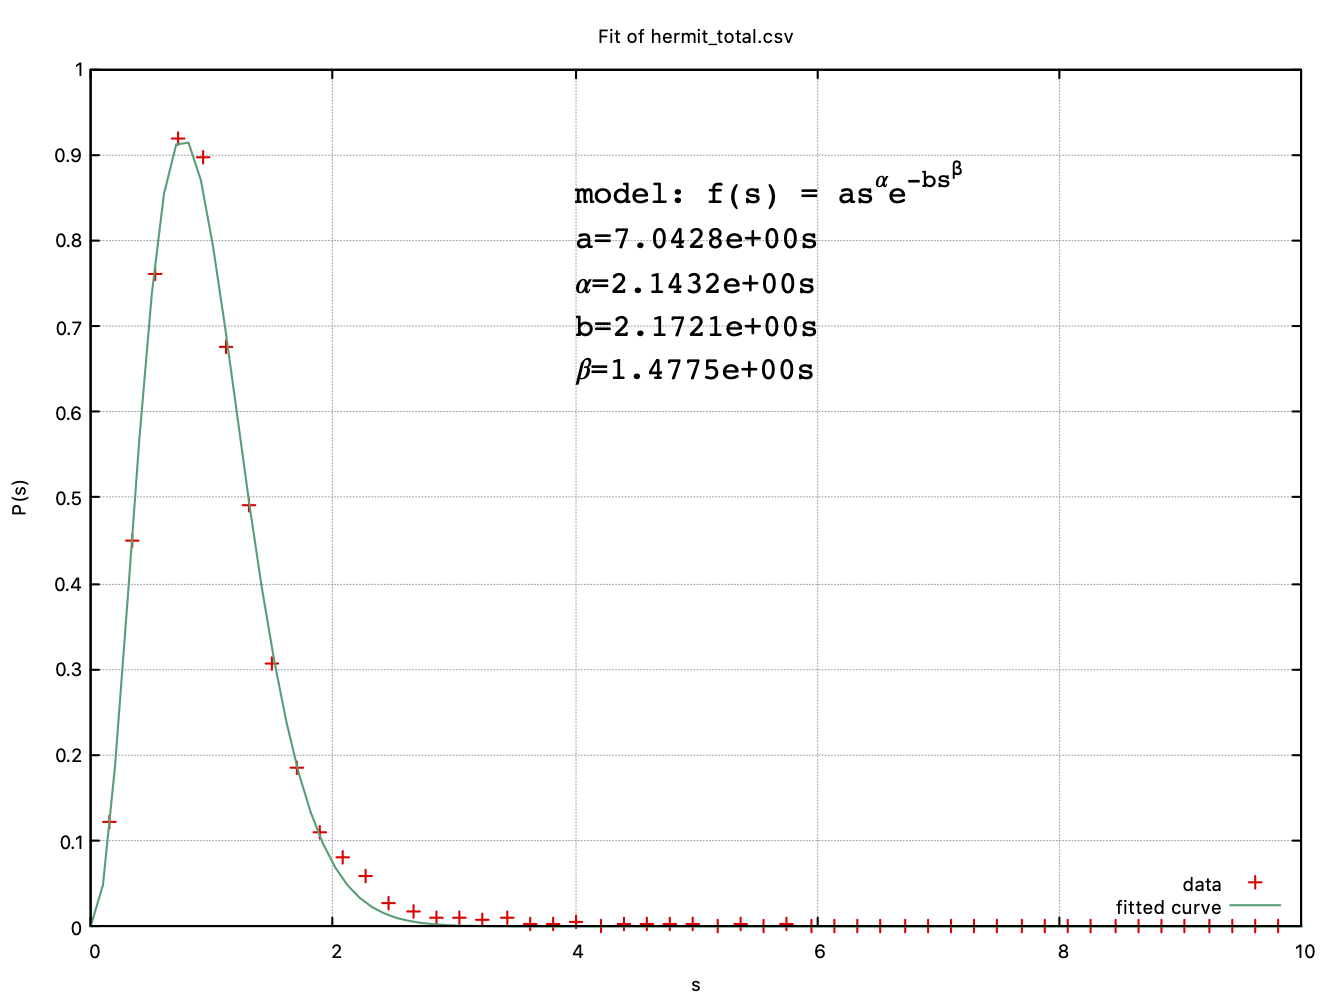
\includegraphics[width=.33\textwidth]{hermitian_total}\hfill
    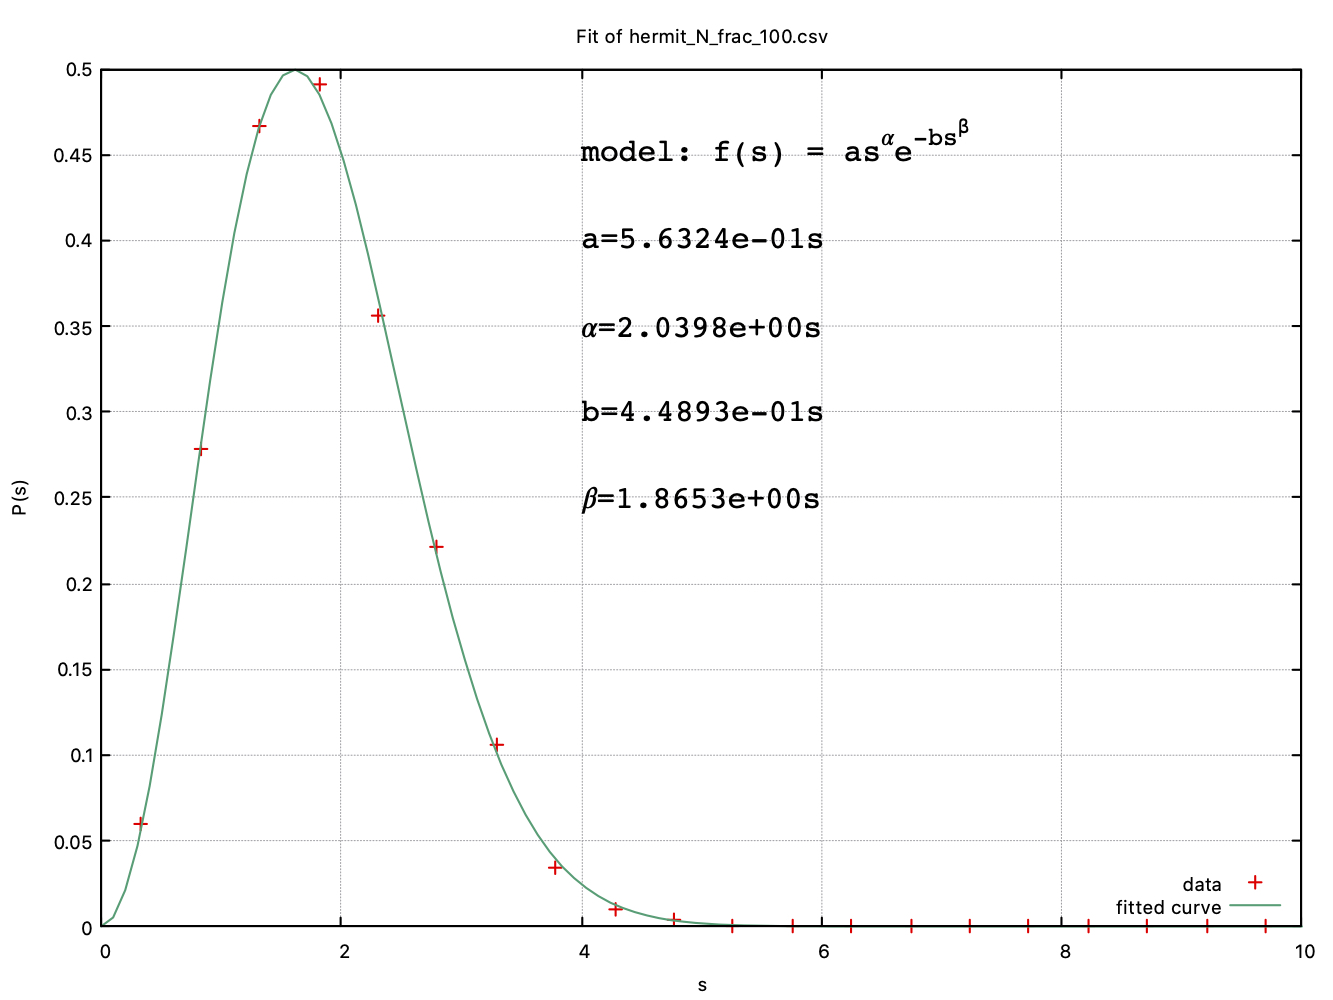
\includegraphics[width=.33\textwidth]{hermitian_N_frac_100}\hfill
    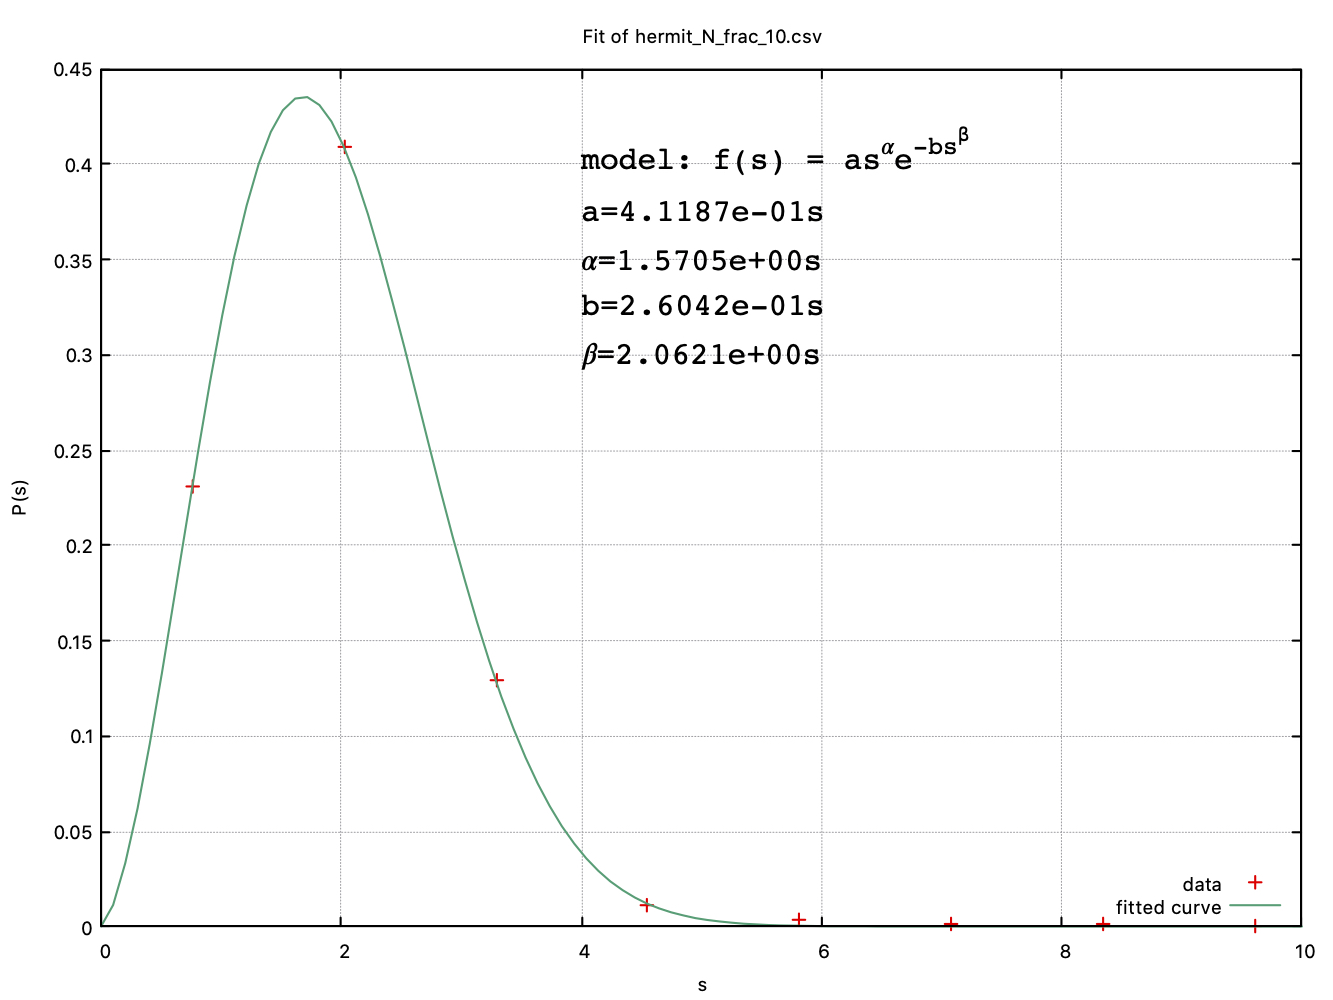
\includegraphics[width=.33\textwidth]{hermitian_N_frac_10}
    \\[\smallskipamount]
    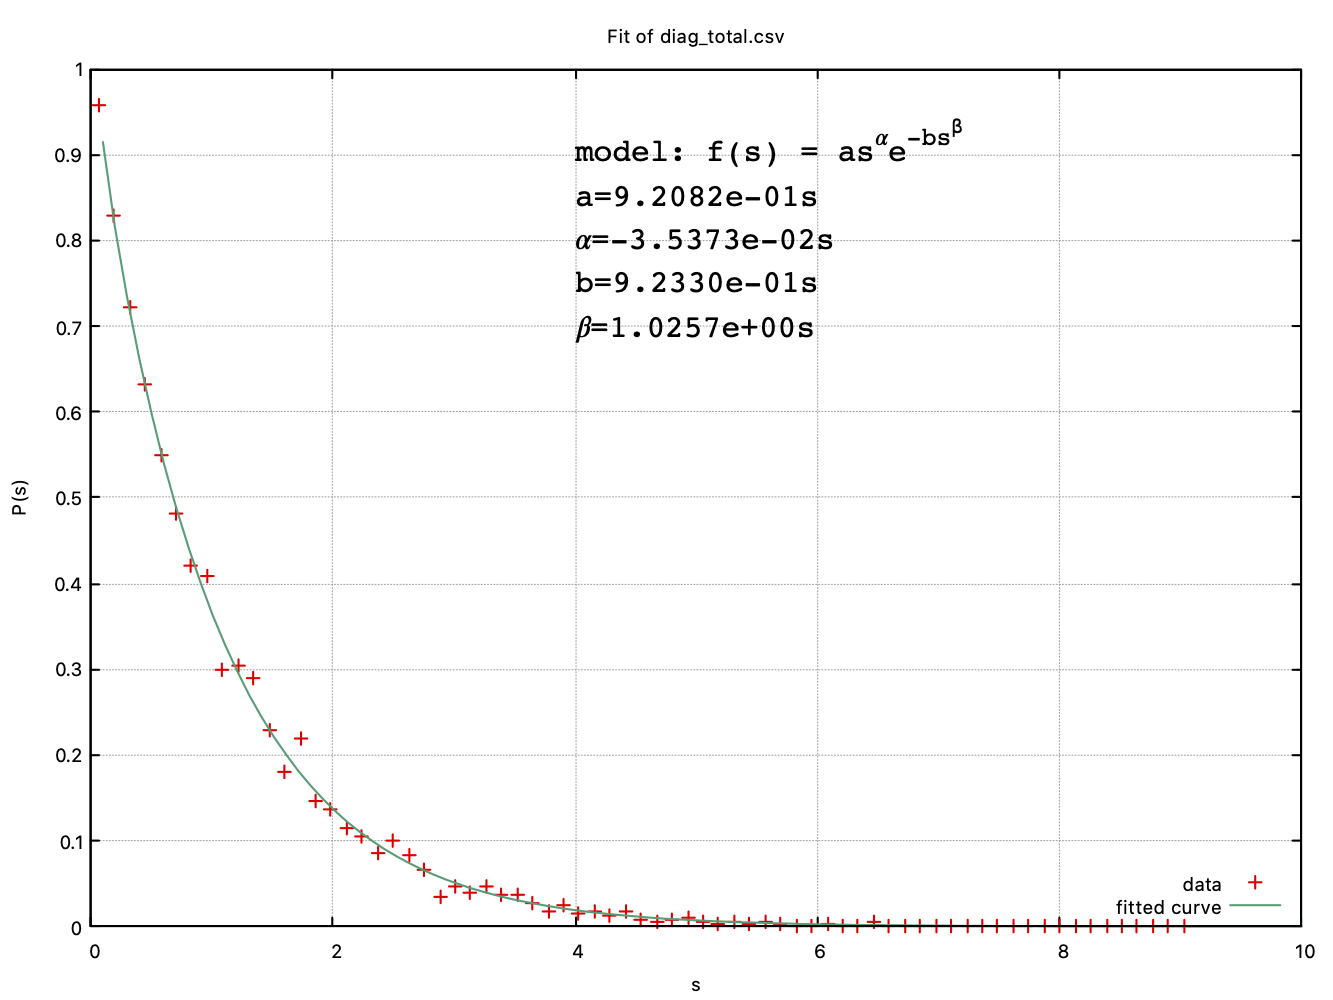
\includegraphics[width=.33\textwidth]{diag_total}\hfill
    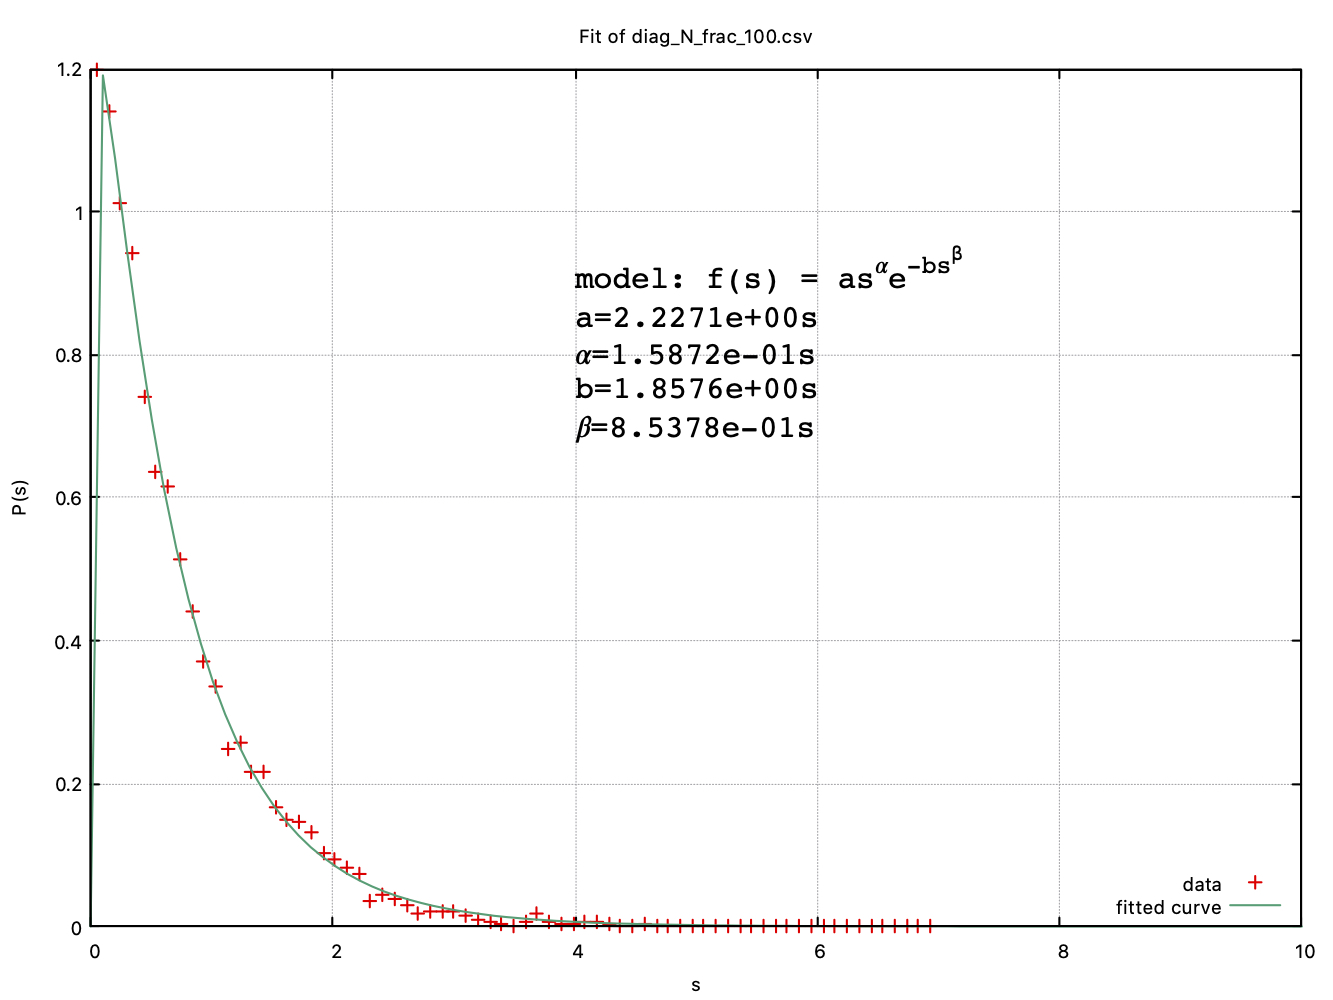
\includegraphics[width=.33\textwidth]{diag_N_frac_100}\hfill
    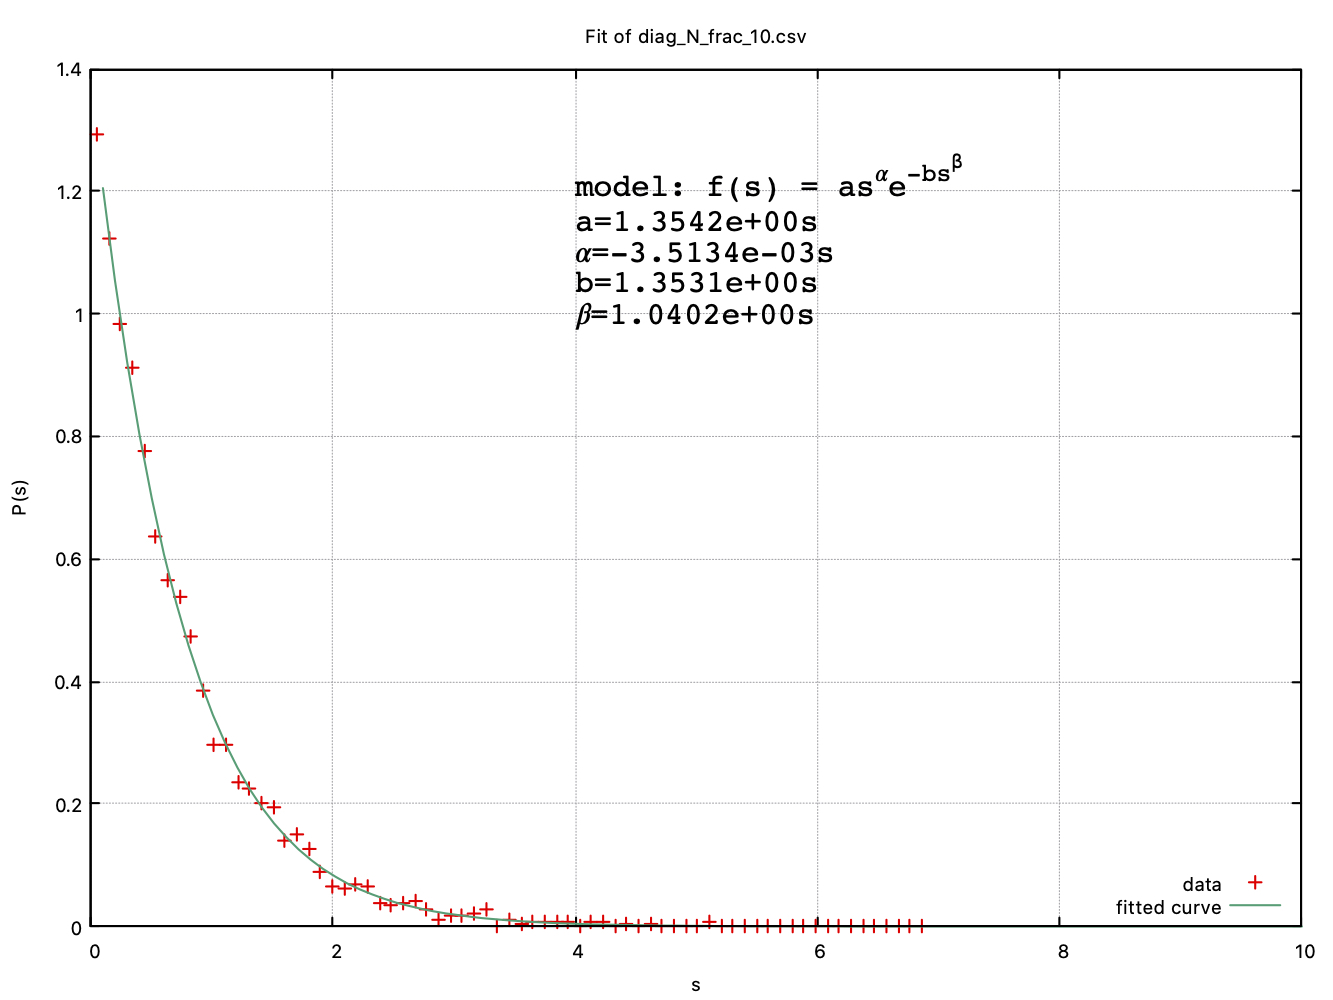
\includegraphics[width=.33\textwidth]{diag_N_frac_10}
    \caption{The three top images are the fits produced with hermitian matrices, the bottom ones are the fit produced with diagonal matrices. From left to right, the quantity $\bar{\Delta\lambda}$ is computed respectively with $N$,$N/100$ and $N/10$ samples, where N is the dimension of the matrix.}\label{fig:foobar}
\end{figure}


The table below reports the <r> values in the cases considered in \ref{fig:foobar}. The results found, seems to be consistent with the only ones that i found in litterature \href{https://arxiv.org/abs/1212.5611v1}{here}.

\begin{table}[H]
\begin{tabular}{l|l|l|l|}
                  & \textbf{total} & \textbf{N/100} & \textbf{N/10} \\ \hline
\textbf{hermitian} & $<r> = 0.597$  & $<r> =0.598$   & $<r> =0.601$  \\ \hline
\textbf{diagonal}  & $<r> =0.381$   & $<r> =0.393$   & $<r> =0.390$
\end{tabular}
\end{table}


\section{Self-evaluation}
I think the main objectives of the exercises are reached. probably, a more in-depth theoretical analysis would have been useful for a more detailed analysis of the obtained results.



\end{document}
